\chapter{Protezione Dati Sensibili}

\section{Introduzione}
Molti Database contengono \textbf{dati sensibili}. La definizione di dato sensibile, e la distinzione dal dato \textbf{personale}, in senso \textbf{giuridico}, è complessa, e dipende dal contesto legislativo in cui si valuta. In particolare in Italia il dato personale viene indicato come un'informazione che permette di identificare un individuo (anagrafica), mentre un dato sensibile rappresenta un'informazione su aspetti della vita privata dell'individuo (orientamento sessuale, opinione politica, credo religioso, etc.). \\

Ai fini pratici della sicurezza informatica definiremo dati sensibili quei dati che \textbf{non dovrebbero essere resi pubblici}. L'identificazione dei dati sensibili dipende molto dal \textbf{database} e dalla sua specifica \underline{applicazione}. I due casi estremi di questa categorizzazione sono: 
\begin{itemize}
\item \underline{Nessun} dato sensibile (ad es. il catalogo di una biblioteca)
\item \underline{Tutti} dati sensibili (ad es. un database della difesa militare)
\end{itemize}
Questi sono i casi più semplici da gestire, in quanto si \underline{garantisce} accesso a tutto il database o si \underline{nega} accesso a tutto il DB. In generale si ha che solo \textbf{alcuni dati sono sensibili} e che, inoltre, ognuno presenta un \textbf{diverso livello di sensibilità} necessario da applicare.

\begin{figure}[htbp]
	\centering
	{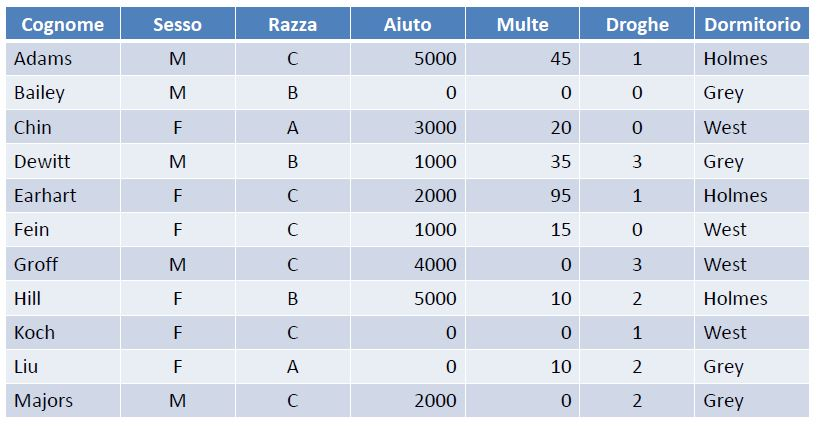
\includegraphics[height=8cm, width=10cm, keepaspectratio]{Immagini/dati_sensibili/prot_dati_01.JPG}}
	\caption{Esempio di una tabella Studente che contiene informazioni sugli studenti di una facoltà\label{fig:tabella_db}}
\end{figure}

Prendiamo come esempio la tabella \textbf{Studente} di fig: \ref{fig:tabella_db}. In questo contesto campi \textbf{non sensibili} risultano essere \textbf{Cognome} e \textbf{Dormitorio}, quelli \textbf{sensibili} sono \textbf{Aiuto}, \textbf{Multe} e \textbf{Droghe} mentre quelli \textbf{parzialmente sensibili} sono \textbf{Sesso} e \textbf{Razza}. La classificazione dei dati come sensibili avviene secondo i seguenti parametri:

\begin{itemize}
	\item \textbf{Sensibili per Contenuto}, in cui è il valore dell'attributo ad essere sensibile.
	\item \textbf{Sensibili per Provenienza}, in questo caso è la fonte dei dati a necessitare riservatezza (e.g. messaggi di un informatore la cui identità segreta verrebbe compromessa se i dati venissero divulgati).
	\item \textbf{Dichiarati Sensibili}, è lo stesso amministratore del sistema a dichiarare che i dati sono sensibili (e.g. donatore anonimo).
\end{itemize}

Le parti sensibili di un dato possono essere un singolo \textbf{attributo} di un record o un intero \textbf{record}. Inoltre la sensibilità di una parte potrebbe essere tale in senso assoluto o dipendere dal resto dei dati: ad esempio, la latitudine di una postazione segreta diventa sensibile se si conosce anche la longitudine, mentre lo stipendio di un dipendente è un dato sensibile a prescindere dal resto delle informazioni divulgate. \\

Il trattamento dei dati sensibili è una materia complicata. Come divulgarli e come proteggerli sono i problemi principali. Va tenuto conto del fatto che, attraverso attacchi inferenziali, è possibile risalire a dati sensibili anche se questi ultimi non vengono divulgati direttamente. Vediamolo con un esempio.
\begin{figure}[htbp]
	\centering
		{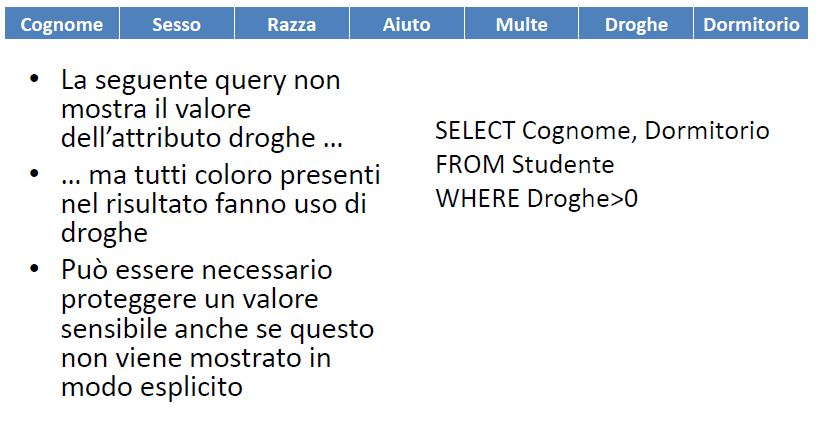
\includegraphics[height=8cm, width=8cm, keepaspectratio]{Immagini/dati_sensibili/prot_dati_02.JPG}}
			\caption{Esempio di come ottenere dati sensibili senza leggerli direttamente \label{fig:query_db}}
\end{figure}

Per evitare questo tipo di attacchi si potrebbe pensare di impedire totalmente l'accesso ai campi sensibili, ad esempio rifiutando ogni tipo di query che faccia riferimento al campo sensibile. Tuttavia ciò limiterebbe anche le interrogazioni legittime.
Emergono quindi due esigenze contrastanti:

\begin{itemize}
	\item Nascondere i dati per evitare di fornire dati sensibili
	\item Facilitare la divulgazione dei dati non sensibili per consentire l'uso corretto di questi da parte degli utenti autorizzati
	\end{itemize}
	
\begin{figure}[htbp]
	\centering
	{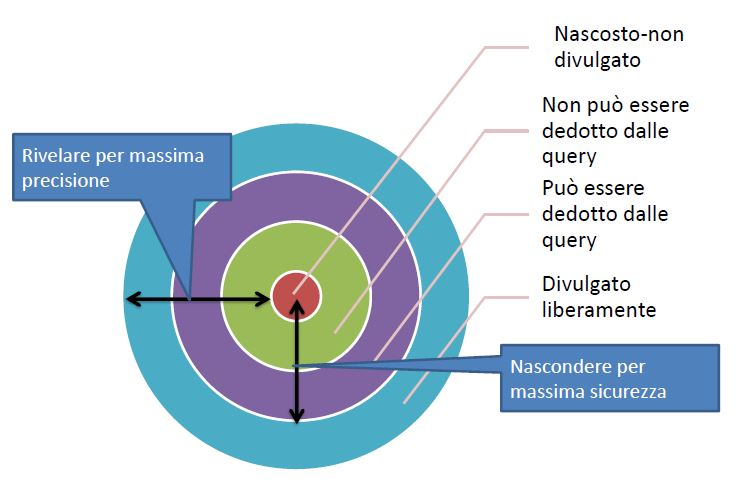
\includegraphics[height=11cm, width=11cm, keepaspectratio]{Immagini/dati_sensibili/prot_dati_03.JPG}}
				\caption{Rappresentazione grafica di accessibilità vs. protezione dei dati \label{fig:protezione_vs_accessibilita}}
\end{figure}

\subsection{Tipi di Divulgazione} 
Esistono diverse modalità di divulgazione di un dato o insieme di dati:

\begin{itemize}
	\item\textbf{Dati Esatti}: consiste nella divulgazione del valore esatto del campo sensibile. Può avvenire per richiesta esplicita o come parte del risultato di una query insieme ad altri dati non sensibili o, addirittura, per errore del sistema
	\item \textbf{Limiti}: si rendono noti gli estremi tra cui varia un dato sensibile (superiore, \textbf{H}, e inferiore, \textbf{L}). Con una ricerca dicotomica si potrebbe arrivare a dedurre un valore molto prossimo a quello esatto. In certi casi, comunque, la semplice conoscenza del fatto che un valore superi o meno una certa soglia rappresenta una violazione alla sicurezza.
	\item \textbf{Risultato Negativo}: a volte l'informazione risiede più che nel valore assoluto di un attributo, nel suo confronto con un altro valore. Sapere che un attributo è diverso da zero, ad esempio, potrebbe di per sé rappresentare una discreta quantità di informazione (se il numero di condanne di una persona non è zero, si sa che quest'ultima è stata condannata almeno una volta).
	\item \textbf{Esistenza}: anche la sola conoscenza di esistenza di un attributo è sensibile (un responsabile del personale potrebbe desiderare che non si sappia che la durata delle interurbane dei dipendenti viene monitorata, quindi la scoperta del campo interurbane in una tabella con i dati del personale rivelerebbe dati sensibili)
	\item \label{par:val_prob} \textbf{Valore Probabile}: tramite l'utilizzo di diverse query e incrociando i dati ottenuti si possono inferire informazioni non precise, ma attendibili, riguardo i valori di alcuni dati sensibili. Ad esempio, se conosciamo l'indirizzo di residenza di tizio, sappiamo che 4 persone risiedono nello stesso indirizzo, e che una persona che risiede in quell'indirizzo è iscritta al partito X possiamo dire che tizio è iscritto al partito X con una probabilità del 25 $\%$.
\end{itemize}

\section{Inferenza}
L'\textbf{Inferenza} è un metodo per dedurre o derivare dati sensibili a partire dai dati non sensibili a disposizione. Esistono due principali categorie di attacchi inferenziali:
\begin{itemize}
	\item Attacchi diretti
	\item Attacchi indiretti
\end{itemize}
\subsection{Attacchi diretti}
Ricordando la tabella di fig. \ref{fig:tabella_db}, la query seguente rappresenta un attacco diretto, ovvero un tentativo diretto di accedere ad un dato sensibile:

\begin{algorithm}
\begin{lstlisting}[caption={Query che sfrutta inferenza per ottenere dati sensibili e viene bloccata}]
SELECT Cognome
FROM Studente
WHERE Sesso = M AND Droghe = 1
\end{lstlisting}
\end{algorithm}

Una query di questo tipo potrebbe essere rifiutata dal DBMS in quanto le tuple del risultato sono quelle con uno specifico valore su un attributo sensibile. La seguente query, invece, intuitivamente risulta legale ma va a selezionare solo tuple sensibili, in quanto la seconda e la terza condizione non sono mai soddisfatte.

\begin{algorithm}
\begin{lstlisting}[caption={Query che sfrutta inferenza per ottenere dati sensibili e non viene bloccata}]
SELECT Cognome
FROM Studente
WHERE (Sesso = M AND Droghe = 1)
	OR (Sesso != M AND Sesso != F)
	OR (Dormitorio = 'Ayres')
\end{lstlisting}
\end{algorithm}

Per scovare l'accesso improprio ai dati, il DBMS dovrebbe capire che ci sono solo due valori ammessi per il campo Sesso e che non c'è alcuna tupla con valore Dormitorio uguale ad 'Ayres'. Per limitare gli Attacchi Diretti è applicata, alle volte, una regola \textit{n elementi sul k percento}, che consiste nel non restituire il risultato di una query se un piccolo numero di elementi divulgati costituisce una grande percentuale del valore restituito (nel caso mostrato come esempio nel paragrafo \ref{par:val_prob} relativo alla divulgazione per valore probabile, fare una query che richiede i residenti ad un dato indirizzo ed iscritti ad un partito dà come risultato un unico elemento che rappresenta il 100\%).

\subsection{Attacchi Indiretti}
Un attacco inferenziale indiretto si basa sulla deduzione di dati sensibile a partire da uno o più dati statistici intermedi (somme, medie o conteggi, spesso divulgate da organizzazioni che mirano alla diffusione di informazioni aggregate e detengono dati sensibili di molto soggetti). In seguito descriveremo diversi tipi di attacchi inferenziali indiretti.

\subsubsection{Somma e Conteggio}

Una query del genere \ref{query:neg} potrebbe sembrare innocua dato che restituisce solo valori aggregati, ma il risultato è una \textbf{Divulgazione di Tipo Negativo}, in quanto è possibile dedurre dal valore nullo nel dormitorio Holmes che le donne in quel dormitorio non ricevono aiuti finanziari (che è un dato decretato sensibile). 

\begin{algorithm} 
\begin{lstlisting}[caption={Query che implementa un attacco con somma per ottenere Divulgazione di tipo negativo \label{query:neg}}] 
SELECT Sesso, Dormitorio, SUM(Aiuto)
FROM Studente
GROUP BY Sesso,Dormitorio
\end{lstlisting}
\end{algorithm}

\begin{figure}[htbp]
	\centering				
		{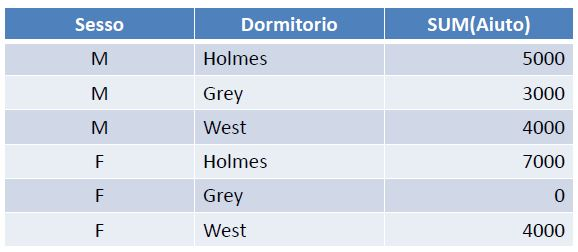
\includegraphics[height=11cm, width=11cm, keepaspectratio]{Immagini/dati_sensibili/prot_dati_09.JPG}}
							\caption{Risultato query ~\ref{query:neg} \label{fig:query_indiretta_result}}                         
\end{figure}

\begin{algorithm}
\begin{lstlisting}[caption={Query che implementa un attacco con conteggio \label{query:count}}] 
SELECT Sesso, Dormitorio, COUNT(*)
FROM Studente
GROUP BY Sesso,Dormitorio
\end{lstlisting}
\end{algorithm}

\begin{figure}[htpb]
	\centering
		{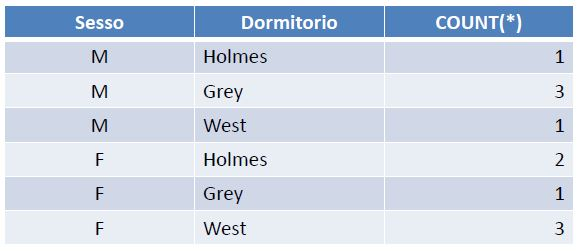
\includegraphics[height=11cm, width=11cm, keepaspectratio]{Immagini/dati_sensibili/prot_dati_08.JPG}}
							\caption{Risultato query ~\ref{query:count} \label{fig:query_indiretta_result1}}                           
\end{figure}

Inoltre, il conteggio può essere combinato con la somma per produrre risultati ancora più rivelatori. Il risultato della query di \textbf{Attacco di Somma} \ref{query:neg} combinata con la query di \textbf{Attacco di Conteggio} \ref{query:count} rivela che i due uomini nel dormitorio Holmes e West ricevono un aiuto finanziario di 5000 e 4000.

\subsubsection{Media}

La media può permettere di ottenere informazioni esatte se utilizzate in combinazione con il conteggio: se riesco ad ottenere la media su un insieme formato da un solo elemento, riesco a conoscere il valore esatto per quell'elemento. Per ovviare a questa minaccia a volte i DBMS implementano meccanismi di sicurezza che impediscono di dilvugare la media calcolata su un numero di elementi al di sotto di una certa soglia. Tuttavia, usati in modo opportuno, gli attacchi con media riescono anche ad aggirare eventuali controlli sulla numerosità dell'insieme su cui viene calcolata. Ad esempio, supponiamo che la media non venga divulgata se la somma degli elementi su cui è calcolata è pari ad 1 (legge interna del DBMS). 

\begin{algorithm}
\begin{lstlisting}[caption={Query di Media per ottenere informazioni sugli studenti del dormitorio Holmes \label{query:avg2}}] 
SELECT AVG(Aiuto)
FROM Studente
WHERE Dormitorio = 'Holmes'

SELECT AVG(Aiuto)
FROM Studente
WHERE Dormitorio = 'Holmes'
	AND Sesso = 'F'
\end{lstlisting}
\end{algorithm}

La prima query di~\ref{query:avg2} restituisce una media di 4000, mentre la seconda restituisce una media di 3500. Conosciamo quindi quanto recepiscono come aiuto, in media, tutti gli studenti e le sole femmine del dormitorio Holmes. Possiamo inoltre aggiungere informazioni di conteggio, utilizzando le query~\ref{query:count2}.

\begin{algorithm}
\begin{lstlisting}[caption={Query di conteggio per ottenere informazioni sugli studenti del dormitorio Holmes \label{query:count2}}]
SELECT COUNT(*)
FROM Studente
WHERE Dormitorio = 'Holmes'

SELECT COUNT(*)
FROM Studente
WHERE Dormitorio = 'Holmes'
	AND Sesso = 'F'
\end{lstlisting}
\end{algorithm}

A questo punto sappiamo che nel dormitorio Holmes risiedono 3 persone, due delle quali femmine. Denominati $a_1,a_2,a_3$ gli aiuti recepiti dai tre individui, possiamo scrivere:

\begin{equation}
\frac{a_1 + a_2 + a_3}{3} = 4000 \Rightarrow a_1 + a_2 + a_3 = 12000
\end{equation}

\begin{equation}
\frac{a_1 + a_2}{2} = 3500 \Rightarrow a_1 + a_2 = 7000
\end{equation}

\begin{equation}
 a_3 = 12000 - (a_1 + a_2) = 5000
\end{equation}

Tramite la procedura illustrata si trova che $ a_{3} = 5000 $, ovvero l'importo esatto dell'unico maschio che risiede nel dormitorio Holmes

\subsubsection{Attacchi di Tracker}
Abbiamo visto che una delle tecniche di protezione dall'inferenza consiste nel non divulgare i dati se un \textbf{piccolo numero di elementi fornisce molta informazione}; è possibile aggirare questa limitazione effettuando più query lecite e combinandole insieme. Vediamolo con un esempio: esaminiamo la query \ref{query:tracker1}.

\begin{algorithm}
\begin{lstlisting}[caption={Esempio di query di tracker non lecita du DB \label{query:tracker1}}] 
SELECT COUNT(*)
FROM Studente
WHERE Razza = 'C'
	AND Sesso = 'F'
	AND Dormitorio = 'Holmes'
\end{lstlisting}
\end{algorithm}

La query \ref{query:tracker1} è, ovviamente, bloccata dal DBMS in quanto va a richiedere un unico risultato sulla tabella del DB in fig. \ref{fig:tabella_db}. Il dato non viene divulgato in quanto \textbf{dominato da una sola tupla}, ma osserviamo che può essere calcolato contando le donne che \textbf{non sono di razza C}, sommando il risultato a quelle che \textbf{non risiedono nel dormitorio Holmes} e infine sottraendo questa somma al numero totale delle femmine. Tale calcolo deriva dalle leggi di De Morgan. Infatti, ponendo:

\begin{itemize}
\item R := (Razza='C')
\item D := (Dormitorio='Holmes')
\item S := (Sesso = 'F')
\end{itemize}

Allora:

\begin{equation}
R \cdot D \cdot S = (R \cdot D) \cdot S =\overline{\overline{(R \cdot D)}} \cdot S
\end{equation}

Per le leggi di De Morgan:
\begin{equation}
\overline{(R \cdot D)} = \overline{R} + \overline{D}
\end{equation}

Allora:
\begin{equation} \label{eq:tracker}
\overline{\overline{(R \cdot D)}} \cdot S = \overline{(\overline{R} + \overline{D})} \cdot S
\end{equation}

Possiamo allora ricavare il risultato desiderato attraverso le query~\ref{query:tracker2}. In particolare il dato si può ricavare sottraendo il risultato della seconda query dal risultato della prima.
\begin{algorithm}
\begin{lstlisting}[caption={Esempio di query di tracker lecita du DB \label{query:tracker2}}] 
SELECT COUNT(*)
FROM Studente
WHERE Sesso = 'F'
	
SELECT COUNT(*)
FROM Studente
WHERE Sesso = 'F'
	AND ( Razza != C
	OR Dormitorio != 'Holmes')
\end{lstlisting}
\end{algorithm}

\subsubsection{Vulnerabilità del Sistema Lineare}
L'attacco di Tracker è un caso specifico di una vulnerabilità più generica in cui sfruttando l'algebra, la logica e un po' di fortuna si riesce ad ottenere tramite diverse query dei valori protetti. Nell'esempio~\ref{query:tracker1} la query protetta è del tipo:

\begin{equation}
q = \parallel (Sesso \: = \: 'F') \wedge (Razza \: = \: 'C') \wedge (Dormitorio \: = \: 'Holmes') \parallel
\end{equation}
In base all'algebra, possiamo riscrivere la query nel seguente modo: 
{\footnotesize
\begin{equation}
q = \parallel (Sesso \: = \: 'F') \parallel - \parallel (Sesso \: = \: 'F') \wedge \neg( (Razza \: = \: 'C') \vee (Dormitorio \: = \: 'Holmes')) \parallel
\end{equation}}
Più in generale potremmo avere le seguenti query:
\newline
\newline
$q_{1} = c_{1} + c_{2} + c_{3} + c_{4} + c_{5}$
\newline
$q_{2} = c_{3} + c_{2} $
\newline
$q_{3} = c_{5} + c_{1} + c_{3}$
\newline
$q_{4} = c_{4} + c_{7} + c_{2}$
\newline
$q_{5} = c_{8} + c_{3}$
\newline
\\
Nessuna delle query rivela un qualsiasi valore $c_{i}$ ma, risolvendo il sistema, possiamo conoscerli tutti.

\subsubsection{Aggregazione}
L'aggregazione è un altro particolare tipo di inferenza, in cui si cerca di ottenere dati sensibili mettendo insieme dati non sensibili (ad esempio il nome di un impiegato e il suo stipendio non sono dati sensibili se considerati separatamente. La loro combinazione invece si). \\

Evitare l'aggregazione è difficile perché bisogna tenere conto delle informazioni già in possesso dell'utente. Se un utente conosce il nome di un dipendente non devo, ad esempio, comunicargli lo stipendio e viceversa. Purtroppo tenere traccia di tutte le informazioni in possesso ad ogni utente è proibitivo. Inoltre utenti diversi potrebbero condividere tutti le informazioni in loro possesso, aiutandosi a vicenda ad aggregare i dati al fine di ricavare informazioni sensibili.

\section{Protezione dall'Inferenza}
Esistono alcune tecniche per combattere l'inferenza:
\begin{itemize}
\item \textbf{Analisi} delle query
\item \textbf{Soppressione} dei valori sensibili per non fornirli
\item \textbf{Occultamento} del valore reale, con un altro simile
\end{itemize}
Tali soluzioni tendono a proteggere un DB dal problema dell'inferenza, ma al tempo stesso limitano anche le
informazioni fornite agli utenti che intendono fare un uso legittimo dei dati.
\subsection{Soppressione}
Un esempio di \textbf{soppressione} è la già citata regola del \textit{n elementi sul k percento}; purtroppo, affinché questo tipo di protezione sia efficace, può essere necessario sopprimere altri dati per evitare che quelli sensibili siano ottenibili per differenza.

\begin{figure}[htpb]
	\centering
		\subfigure[Numero di residenti per Sesso e Dormitorio]
		{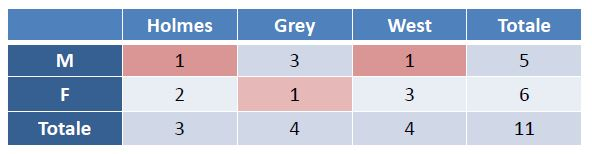
\includegraphics[height=2cm, width=8cm, keepaspectratio]{Immagini/dati_sensibili/prot_dati_15.JPG}}
		
		\subfigure[Tabella dopo la soppressione. Si noti come i dati sopressi possono essere comunque ricavati per differenza]
		{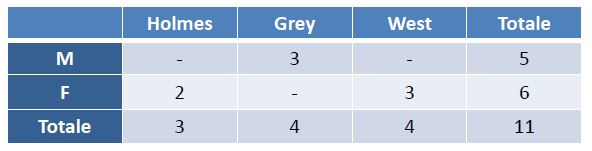
\includegraphics[height=2cm, width=8cm, keepaspectratio]{Immagini/dati_sensibili/prot_dati_16.JPG}}
				
		\caption{Esempio di protezione per soppressione
		  \label{fig:query_soppressione}}  

\end{figure}


\subsection{Occultamento}

\subsubsection{Utilizzo di dati combinati}
Per evitare di divulgare dati sensibili è possibile combinare più righe o colonne, come riportato in fig.~\ref{fig:query_occultamento}.

\begin{figure}[htpb]
	\centering
		\subfigure[Numero di residenti per Sesso e Uso di Droghe]
		{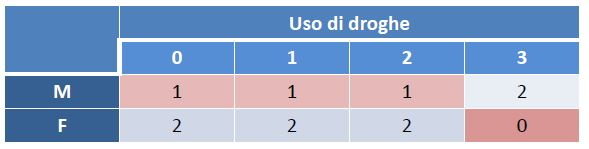
\includegraphics[height=2cm, width=8cm, keepaspectratio]{Immagini/dati_sensibili/prot_dati_17.JPG}}
		
		\subfigure[Tabella dopo l'occultamento]
		{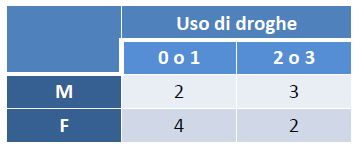
\includegraphics[height=2cm, width=8cm, keepaspectratio]{Immagini/dati_sensibili/prot_dati_18.JPG}}
				
		\caption{Esempio di protezione per occultamento
		  \label{fig:query_occultamento}}  

\end{figure}

\subsubsection{Campione Casuale dei dati}

Alternativamente la query può essere eseguita su di un \textbf{Campione Casuale} dei dati, in cui il campione deve essere abbastanza ampio da rappresentare l'intera popolazione. In questo modo i dati sono sempre rappresentativi ma si diminuisce la possibilità di attacchi statistici.

\subsubsection{Perturbazione Casuale dei dati}

A volte può essere utile perturbare i valori del database con un piccolo errore: per ogni $x_{i}$ che rappresenta il valore vero dell'attributo \textit{i} si può generare un piccolo errore $e_{i}$ e aggiungerlo a $x_{i}$ per calcolare dati statistici.
Valori di query aggregate, quali la somma o la media, produrranno valori vicini a quelli veri ma non esatti.

\section{Esercitazione sull'inferenza}
Con riferimento alla tabella dipendenti, in \figurename ~\ref{fig:Tabella_dipendenti}, trovare lo stipendio di Mister X con un attacco indiretto di tipo media.
\begin{figure}[htbp]
	\centering%
	\subfigure%
	{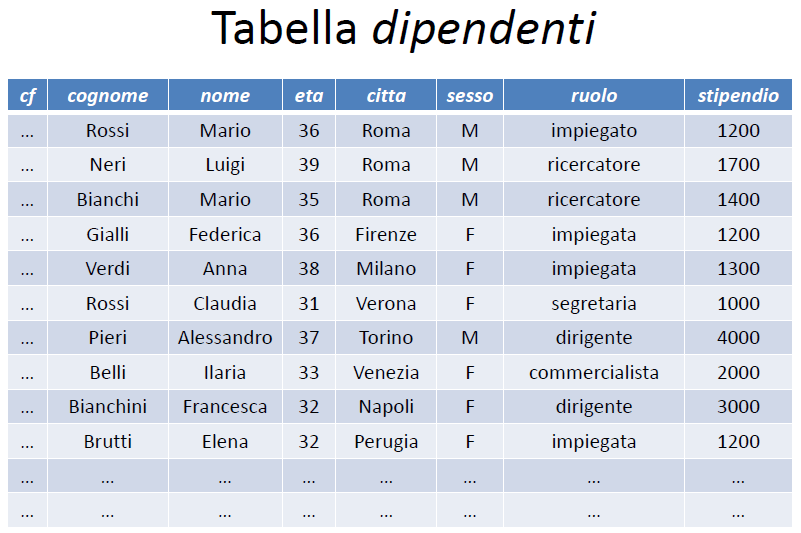
\includegraphics[height=8cm, width=12cm, keepaspectratio]{Immagini/dati_sensibili/Tabella_dipendenti.png}}
	\caption{Tabella dipendenti\label{fig:Tabella_dipendenti}} 	
\end{figure}
\\
Si hanno a disposizione le seguenti informazioni:
\begin{enumerate}
\item [a.] Mister X è un uomo con più di 30 anni e non è di Roma;
\item [b.] i rimanenti dipendenti maschi con più di 30 anni sono tutti romani;
\item [c.] nessun dipendente donna è di Roma.
\end{enumerate}
Si tenga conto, inoltre, che viene applicata la seguente politica di protezione dei dati sensibili:
\begin{enumerate}
\item il campo stipendio non può essere divulgato direttamente e non può essere utilizzato come criterio di filtraggio;
\item i criteri di filtraggio possono essere \emph{età}, \emph{sesso}, e \emph{città};
\item non possono essere utilizzati più di due criteri di filtraggio in una singola interrogazione;
\item è consentita la divulgazione di medie e conteggi a patto che si riferiscano ad almeno tre tuple.
\end{enumerate}
\subsection{Svolgimento}
\subsubsection{Idea base}
Una possibile strategia di attacco prevede l'individuazione di due insiemi di tuple U e V tali che:
\begin{enumerate}
\item [I.] ciascun insieme contiene singolarmente almeno tre tuple (vincolo 4.);
\item [II.] ciascun insieme deve poter essere individuato usando al più due condizioni di filtraggio (vincolo 3.) basate sugli attributi eta, sesso, e città (vincolo 2.);
\item [III.] la differenza insiemistica $U \setminus V$ deve contenere soltanto mister X; ovvero ${Mister X} = U \setminus V$;
\item [IV.] l'insieme $V$ deve essere un sottoinsieme di $U$, i.e. $V \subset U$
\end{enumerate}
Una volta individuati due insiemi $U$ e $V$, soddisfacenti le condizioni I, II, III e IV, ponendo:
\begin{itemize}
\item $m_{U}$ = media degli stipendi dei dipendenti in $U$;
\item $c_{U}$ = numero dei dipendenti in $U$;
\item $m_{V}$ = media degli stipendi dei dipendenti in $V$;
\item $c_{V}$ = numero dei dipendenti in $V$;
\end{itemize}
si ottiene che: $stipendio_{Mister X} = m_{U} \cdot c_{U} - m_{V} \cdot c_{V}$.\\
\subsubsection{Individuazione di $U$ e $V$}
A questo punto si considerino i seguenti insiemi:
\begin{itemize}
\item $A$: insieme dei dipendenti di sesso maschile (sesso = M);
\item $B$: insieme dei dipendenti con più di 30 anni (eta > 30);
\item $C$: insieme dei dipendenti romani (città = Roma);
\end{itemize}
Si osservi che dalla (a) e dalla (b) risulta che: ${Mister X} = (A \cap B) \setminus C = (A \cap B) \setminus (B \cap C)$\\
mentre dalla (c) si ha che: $C \subset A$\\
pertanto risulta che: ${Mister X} = (A \cap B) \setminus (B \cap C)$ e $(B \cap C) \subset (A \cap B)$\\
quindi gli insiemi $U$ e $V$ sono:
\begin{itemize}
\item $U = A \cap B$
\item $V = B \cap C$
\end{itemize}
\subsubsection{Query SQL}
Infine vediamo quali sono le query  SQL per ottenere le informazioni che ci servono:\\ \\
Individuazione di $m_{U}$ e $c_{U}$:
\begin{lstlisting}
SELECT avg(stipendi), count(stipendi) 
FROM dipendenti 
WHERE sesso = 'M' AND eta > 30;
\end{lstlisting}
Individuazione di $m_{V}$ e $c_{V}$:
\begin{lstlisting}
SELECT avg(stipendi), count(stipendi) 
FROM dipendenti 
WHERE eta > 30 AND citta = 'Roma';
\end{lstlisting}


